Dette afsnit præsenterer Riemann-integralet.\footnote{Afsnittet er baseret på \cite{Abbott2002}, s. 186-204, medmindre andet er angivet.}
Det skal dog bemærkes, at vi ikke benytter Riemanns originale definition, men derimod en videreudvikling af den franske matematiker Darboux.
Det kan bevises, at de to definitioner på integralet er ækvivalente.\footnote{\cite{Bartle2010}, s. 231-232.}

\subsection{Inddelinger samt over- og undersummer}%
  \label{sub:Inddelinger samt over- og undersummer}

Vi starter med nogle grundlæggende definitioner, vi har brug for til at definere integralet.
\begin{definition}[label=def:inddeling]{Inddeling}{}
  Antag $a,\;b \in \mathbb{R}$ sådan at $a <b$.
  Ved en inddeling $P$ af $[a;b]$ forstår vi en endelig mængde $\{x_0,\dotsc, x_n\}$, hvor
  \[
  a=x_0<x_1<\cdots<x_n=b,
  \] 
  og vi skriver 
  \[
  \Delta x_i=x_i-x_{i-1} \quad (i=1,\ldots ,n).
  \]  
\end{definition}
Med en inddeling kan vi dele intervallet $[a;b]$ op i $n$ delintervaller, hvor det $i$'te delinterval har længden $\Delta x_i$:
\[
[a;b]=[x_0;x_1] \cup [x_1;x_2]\cup \cdots \cup [x _{n-1};x_n].
\] 
Vi vil nu definere over- og undersummen af en funktion med hensyn til en given inddeling.

\begin{definition}[label=def:oversum]{Over- og undersum}{}
  Antag $f:[a;b] \to \mathbb{R}$ er en begrænset funktion, og $P=\{x_0,\ldots, x_n\}$ er en inddeling af $[a;b]$. 
  Lad 
  \[
  M_i=\sup \{ f(x):x \in [x _{i-1};x_i] \} \quad{\text{og}} \quad m_i=\inf \{ f(x):x \in [x _{i-1};x_i] \}.
  \] 
  Så er oversummen af $f$ med hensyn til $P$ defineret ved
  \[
  U(f, P)=\sum_{i=1}^{n} M_i \Delta x_i.
  \] 
  Tilsvarende er undersummen af $f$ med hensyn til $P$ defineret ved
  \[
  L(f, P)=\sum_{i=1}^{n} m_i \Delta x_i.
  \] 
\end{definition}

Vi kræver i definitionen, at $f(x)$ er begrænset, da vi så fra supremum- og infimum-egenskaben (sætning \ref{theo:supremum-egenskab} og \ref{theo:infimum-egenskab}) ved, at $M_i$ og $m_i$ eksisterer. 

\begin{theorem}[label=theo:ulighed_overundersum]{Uligheder med over- og undersummer}{}
  Antag $f:[a;b] \to \mathbb{R}$ er en begrænset funktion og $P$ og $P'$ er inddelinger af $[a;b]$ sådan at $P \subseteq P'$. Så gælder
  \[
  L(f, P)\leq L(f, P') \leq  U(f, P') \leq U(f, P).
  \] 
\end{theorem}
\begin{proof} 
  \footnote{Beviset er baseret på \cite{Axler2020}, s. 3-4.} 
  Lad $P=\{ x_0,\ldots , x_n \} $ og $P'=\{x_0',\ldots x_N'\}$. 
  Siden $P \subseteq P'$, så har vi, at for hver $j=1,\ldots , n$ eksisterer $k \in \{ 0,\ldots , N-1 \} $ og $m \in \mathbb{Z}^+$ sådan at $x _{j-1} =x_k'< \cdots < x _{k+m}'=k_j$.

  Så gælder for hver $i=1, \ldots , m$, at ${\{ f(x):x \in [x'_{k+i-1};x'_{k+i }] \} \subseteq \{ f(x):x \in [x_{j-1},x_j]\}  }$, og 
  \begin{equation*}
  \begin{split}
   m_j&=\inf \{ f(x):x \in [x_{j-1};x_j]\} \\
    &\leq  \inf \{ f(x):x \in [x'_{k+i-1};x'_{k+i }] \}\\
    &=m'_{k+i}.
  \end{split}
  \end{equation*}
Vi får så uligheden 
\begin{equation*}
\begin{split}
  m_j \Delta x_j&=\sum_{i=1}^{m} m_j \Delta x _{k+i}\\
  &\leq \sum_{i=1}^{m} m' _{k+i} \Delta x _{k+i}.
\end{split}
\end{equation*}
  Det følger, at $L(f, P) \leq L(f, P')$. 

  Tilsvarende har vi for hver $i=1,\ldots, m$ også, at
  \begin{equation*}
  \begin{split}
    M_j&=\sup \{ f(x):x \in [x_{j-1};x_j] \} \\
    &\geq \sup \{ f(x):x \in [x'_{k+i-1};x'_{k+i}] \} \\
    &=M'_{k+i},
  \end{split}
  \end{equation*}
  og vi får uligheden
  \begin{equation*}
  \begin{split}
  M_j \Delta x_j&=\sum_{i=1}^{m} M_j \Delta x _{k+i}\\
  &\leq \sum_{i=1}^{m} M' _{k+i} \Delta x _{k+i}.
  \end{split}
  \end{equation*}
  Det følger, at $U(f, P) \geq U(f, P')$.

  Siden infimum af en mængde altid er mindre end eller lig med supremum af mængden, så må der til sidst også gælde, at $L(f, P')\leq U(f, P')$.
\end{proof}

 Sætning \ref{theo:ulighed_overundersum} fortæller, at når vi tilføjer ekstra punkter til en inddeling så bliver undersummen potentielt større, og oversummen bliver potentielt mindre.
 Figur \ref{fig:ulighed_overundersum} tydeliggør i høj grad ideen i beviset.

\begin{figure}[H]
\begin{center}
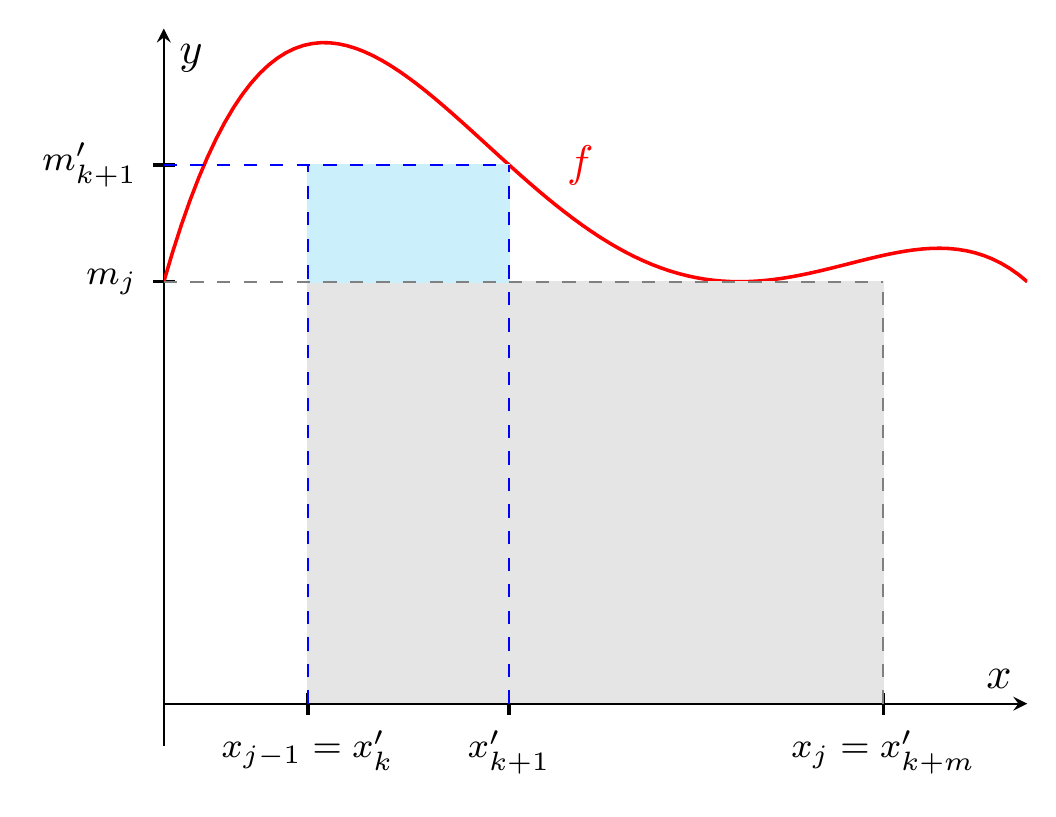
\begin{tikzpicture}[scale=1.6, transform shape]
\begin{axis}[xmin=0, xmax=3, ymin=-0.5, ymax=8, axis lines=middle,
  xlabel=$x$,ylabel=$y$,
  xtick={0.5,1.2,2.5},
  xticklabels={$x _{j-1}=x'_{k}$, $x'_{k+1}$, $x_j=x'_{k+m}$},
  xticklabel style={anchor=north, font=\footnotesize},
  ytick={6.3824,5},
  yticklabels={$m'_{k+1}$, $m_j$},
  every major tick/.append style={thick, major tick length=5pt, black},
  yticklabel style={anchor=east, font=\footnotesize}
  ]
  \addplot[color=red, domain=0:3, samples=100, thick]{-(x-2)^4 - (x-2)^3 + 2*(x-2)^2+5} node[above=5pt, pos=0.7] {$f$};
  \filldraw[gray!20] (axis cs:0.5,0.02) rectangle (axis cs:2.5,5);
  \filldraw[cyan!20] (axis cs:0.5,5) rectangle (axis cs:1.2,6.3824);
  \draw[color=blue, dashed] (axis cs:0.5,0) -- (axis cs:0.5,6.3824);
  \draw[color=blue, dashed] (axis cs:0,6.3824) -- (axis cs:1.2,6.3824);
  \draw[color=gray, dashed] (axis cs:2.5,0) -- (axis cs:2.5,5);
  \draw[color=gray, dashed] (axis cs:0,5) -- (axis cs:2.5,5);
  \draw[color=blue, dashed] (axis cs:1.2,0) -- (axis cs:1.2,6.3824);
\end{axis}
\end{tikzpicture}
\end{center}
  \caption{Ideen i beviset af sætning \ref{theo:ulighed_overundersum}}%
\label{fig:ulighed_overundersum}
\end{figure}

Det næste resultat viser, at der for en reel funktion med definitionsmængden $[a;b]$ gælder, at undersummen mht. enhver inddeling af $[a;b]$ altid er mindre end eller lig med oversummen mht. enhver inddeling af $[a;b]$.

\begin{theorem}[label=theo:undersum_leq_oversum]{Undersum $\leq $ oversum }{}
  Antag $f:[a;b] \to \mathbb{R}$ er en begrænset funktion og $P_1 $ og $P_2$ er inddelinger af $[a;b]$.
  Så gælder
  \[
  L(f, P_1) \leq U(f, P_2).
  \] 
\end{theorem}
\begin{proof} 
  Lad $P_3=P_1 \cup P_2$.
  Så har vi fra sætning \ref{theo:ulighed_overundersum}, at 
  \begin{equation*}
  \begin{split}
    L(f, P_1) &\leq L(f, P_3) \\
    &\leq U(f, P_3)\\
    &\leq U(f, P_2).
  \end{split}
  \end{equation*}
\end{proof}

\subsection{Integrabilitet}%
  \label{sub:Integrabilitet}

Vi har nu set, at når vi tilføjer ekstra punkter til en inddeling så bliver undersummen potentielt større, og oversummen bliver potentielt mindre.
Derudover er en undersum for en funktion altid mindre end en oversum, uanset mht. hvilken inddeling.
Mængden af alle oversummer er så opad begrænset og mængden af alle undersummer er så nedad begrænset. 
Derfor eksisterer supremum for mængden af alle oversummer og ligeledes eksisterer infimum for mængden af alle undersummer.
Vi definerer det såkaldte øvre integral og nedre integral ud fra dette faktum.

\begin{definition}[label=def:øvre_nedre_integral]{Øvre integral, nedre integral}{}
  Antag $f:[a;b] \to \mathbb{R}$ er en begrænset funktion, og lad $\mathfrak{P}$ være mængden af alle inddelinger af $[a;b]$.
  Så er det øvre integral af $f$ defineret ved
  \[
  \upint_{a}^{b} f = \inf \{ U(f, P):P \in \mathfrak{P} \}.
  \] 
  Tilsvarende er det nedre integral af $f$ defineret ved
  \[
  \lowint_{a}^{b} f = \sup \{ L(f, P):P \in \mathfrak{P} \}.
  \] 
\end{definition}

Det viser sig, at det nedre integral for en funktion altid er mindre end eller lig det øvre intagral for funktionen.

\begin{theorem}[label=theo:Nedre_int_leq_øvre_int]{Nedre integral $\leq$ øvre integral }{}
  Antag $f:[a;b] \to \mathbb{R}$ er en begrænset funktion. 
  Så gælder
  \[
  \lowint_{a}^{b} f \leq \upint_{a}^{b} f  
  \]
\end{theorem}
\begin{proof} 
  \footnote{Øvelse 7.2.1 i \cite{Abbott2002}, s. 190.}
  Fra sætning \ref{theo:undersum_leq_oversum} har vi, at $L(f,P_1) \leq U(f,P_2) \text{ for alle }P_1, P_2 \in \mathfrak{P}$.
  Fra definitionen af supremum (def. \ref{def:sup}) følger det så, at 
\begin{equation*}
\begin{split}
  \lowint_{a}^{b} f &= \sup \{ L(f, P) : P \in \mathfrak{P}\} \\
  &\leq U(f, P_2),
\end{split}
\end{equation*}
  hvor $P_2 \in \mathfrak{P}$.
  $\lowint_{a}^{b} f $ er da et undertal for mængden $\{ U(f, P): P \in \mathfrak{P}\} $, og siden infimum af en mængde altid er større end eller lig ethvert undertal for mængden, så har vi
  \begin{equation*}
  \begin{split}
    \lowint_{a}^{b} f &\leq \inf \{ U(f, P): P \in \mathfrak{P} \} \\
    &=\upint_{a}^{b} f.  
  \end{split}
  \end{equation*}
\end{proof}

Ved Riemann-integration arbejder vi kun med funktioner, hvor det øvre og nedre integral har en fælles værdi.
Da vi i dette afsnit kun arbejder med Riemann-integralet og ikke andre integralbegreber, nøjes vi med at sige, at en funktion er integrabel, når den er Riemann-integrabel.
Ligeledes kalder vi blot Riemann-integralet af en funktion for integralet af funktionen.

\begin{definition}[label=def:integrabel]{Integrabel, integral}{}
  Antag $f:[a;b] \to \mathbb{R}$ er en begrænset funktion. 
  Så er $f$ integrabel, hvis
  \[
  \lowint_{a}^{b} f = \upint_{a}^{b} f,   
  \] 
  og denne fælles værdi kaldes for integralet af $f$ fra $a$ til $b$, som denoteres 
  \[
  \int_{a}^{b} f \text{ eller }  \int_{a}^{b} f(x) \,dx.
  \] 
\end{definition}

Bemærk, at den sidste notation for integralet ikke bidrager med nogen ny information ift. den første.
 Integrationsvariablen ($x$) kan nemlig lige så godt repræsenteres af et andet bogstav.
Vi vil da primært benytte den første notation for integralet.

\begin{example}[label=exa:Riemann-integrabel]{Riemann-integrabel funktion}{}
  Lad funktion $f:[0; 1] \to \mathbb{R}$ være defineret ved
  \[
  f(x)=\pi.
  \]
  Det er klart, at arealet under grafen for $f$ må være $\pi $.
  Vi vil nu vise, at funktionen er integrabel, og at integralet af $f$ fra $0$ til $1$ har denne værdi.

  Siden funktionsværdien er konstant, har vi for enhver inddeling $P=\{ x_0, \ldots , x_n \} $ af $[0;1]$, at alle $M_i=m_i=\pi $.
  Oversummerne bliver så
  \begin{equation*}
  \begin{split}
    U(f, P)&=\sum_{i=1}^{n} M_i \Delta x_i \\
    &= \pi \sum_{i=1}^{n} \Delta x_i \\
    &= \pi.
  \end{split}
  \end{equation*}
Tilsvarende bliver undersummerne
  \begin{equation*}
  \begin{split}
    U(f, P)&=\sum_{i=1}^{n} m_i \Delta x_i \\
    &= \pi \sum_{i=1}^{n} \Delta x_i \\
    &= \pi.
  \end{split}
  \end{equation*}
  Vi har altså $\{ U(f, P):P \in \mathfrak{P}\} =\{ L(f, P):P \in \mathfrak{P} \} =\{ \pi  \} $. 
  Det er klart, at $\upint_{0}^{1} f = \lowint_{0}^{1} f =\pi $.
  Således er funktionen integrabel, og integralet bliver da
  \[
  \int_{0}^{1} f = \pi. 
  \] 
\end{example}


Det er imidlertid lidt vanskeligt at bevise, om en funktion er integrabel eller ej alene ud fra definition \ref{def:integrabel}.
Den næste sætning viser da, at en funktion er integrabel præcis når forskellen på undersum og oversum kan gøres vilkårligt lille.

\begin{theorem}[label=theo:integrabilitetskriterie]{Kriterie for integrabilitet}{}
  Antag $f:[a;b] \to \mathbb{R}$ er en begrænset funktion. 
  Så er $f$ integrabel præcis når der for alle $\varepsilon >0$ eksisterer en inddeling $P _{\varepsilon }$ af $[a;b]$, sådan at 
  \[
  U(f, P _{\varepsilon }) - L(f, P _{\varepsilon }) < \varepsilon.    
  \] 
\end{theorem}
\begin{proof} 
  Antag først, at $f$ er integrabel, altså at $\upint_{a}^{b} f  =\lowint_{a}^{b} f $.
  Siden $\upint_{a}^{b} f  $ er infimum af mængden af alle oversummer, så har vi for enhver given $\varepsilon >0$, at der eksisterer en inddeling $P_1$ af $[a;b]$ sådan at
  \[
  U(f, P_1) < \upint_{a}^{b} f + \frac{\varepsilon }{2}, 
  \] 
  for ellers ville $\upint_{a}^{b} f + \frac{\varepsilon }{2}  $ være et undertal. 

  \noindent Ligeledes er $\lowint_{a}^{b} f $ supremum af mængden af undersummer, og der eksisterer en inddeling $P_2$ af $[a;b]$ sådan at
  \[
  L(f, P_2) > L(f) - \frac{\varepsilon }{2}.
  \] 
  Lad $P _{\varepsilon }=P_1 \cup P_2$, så har vi fra sætning \ref{theo:ulighed_overundersum}, at 
  \begin{equation*}
  \begin{split}
    U(f, P _{\varepsilon }) - L(f, P _{\varepsilon }) &\leq U(f, P_1) - L(f, P_2)\\
    &<\left(\upint_{a}^{b} f + \frac{\varepsilon }{2}  \right) - \left(\lowint_{a}^{b} f - \frac{\varepsilon }{2} \right) \\
    &=\frac{\varepsilon }{2} + \frac{\varepsilon }{2}\\
    &=\varepsilon. 
  \end{split}
  \end{equation*}
Lighedstegnet på anden sidst linje kommer fra $f$'s integrabilitet.

  Omvendt, antag nu, at der for enhver given $\varepsilon >0$ eksisterer en inddeling $P _{\varepsilon }$ af $[a;b]$, sådan at 
\[
  U(f, P _{\varepsilon }) - L(f, P _{\varepsilon }) < \varepsilon. 
\] 
  Der gælder så også, at 
  \[
  \upint_{a}^{b} f - \lowint_{a}^{b} f \leq U(f, P _{\varepsilon }) - L(f, P _{\varepsilon }).
  \]
Antag, at $f$ ikke er integrabel, hvilket vil sige, at $\upint_{a}^{b} f \neq \lowint_{a}^{b} f $.
Så har vi $\upint_{a}^{b} f - \lowint_{a}^{b} f >0$.
  Men så kan vi vælge $\varepsilon =\upint_{a}^{b} f - \lowint_{a}^{b} f$, hvilket fører til modstrid, fordi vi så får $\varepsilon  \leq U(f, P _{\varepsilon }) - L(f, P _{\varepsilon })$.
  Således er $f$ integrabel. 
\end{proof}

Med dette kriterie for integrabilitet kan vi bevise, om bestemte funktioner, eller typer af funktioner er integrable.
Det næste vigtige resultat viser, at alle kontinuerte funktioner på lukkede intervaller er integrable.

\begin{theorem}[label=theo:kontinuert_integrabel]{Kontinuert funktion på lukket interval er integrabel}{}
  Antag funktionen $f:[a;b] \to \mathbb{R}$ er kontinuert på $[a;b]$. 
  Så er $f$ integrabel. 
\end{theorem}
\begin{proof} 
  Siden $f$ er kontinuert på $[a;b]$, så følger det fra sætning \ref{theo:kontinuert_begrænset} og \ref{theo:kontinuert_uniform}, at $f$ er begrænset og uniform kontinuert i $[a;b]$. 
  Lad $\varepsilon > 0$ være givet, og lad 
  \[
  \gamma = \frac{\varepsilon }{b-a}.
  \] 
  Så har vi $\gamma >0$, fordi vi har $a<b$. 
  Siden $f$ er uniform kontinuert på $[a;b]$, så eksisterer $\delta >0$ sådan at når $p, q \in [a;b]$ og $\abs{p-q} < \delta  $, så gælder
  \[
  \abs{f(p)-f(q)} < \gamma.
  \] 
  Lad $P _{\varepsilon }=\{ x _{0}, \ldots , x_n \} $ være en inddeling af $[a;b]$, hvor $\Delta x_i < \delta  $ for $i=1, \ldots , n$. 
  Fra sætning \ref{theo:kontinuert_maks} følger det så, at der i hvert delinterval eksisterer $p_i, q_i \in [x_{i-1}; x _{i}]$ sådan at
  \[
  f(p_i)=\sup \{ f(x): x \in [x _{i-1};x _{i}]\} = M_i \text{ og } f(q_i)=\inf \{ f(x): x \in [x _{i-1};x _{i}]\} = m_i
  \] 
  Siden $\abs{p_i - q_i} \leq \Delta x_i < \delta$, så har vi 
\[
  M_i-m_i = f(p_i) - f(q_i) < \gamma. 
\] 
Forskellen på over- og undersummen af $f$ med hensyn til $P _{\varepsilon }$ bliver så
\begin{equation*}
\begin{split}
  U(f, P _{\varepsilon }) - L(f, P _{\varepsilon }) &= \sum_{i=1}^{n} M_i \Delta x_i - \sum_{i=1}^{n} m_i \Delta x_i\\
  &=\sum_{i=1}^{n} \left(M_i - m_i\right) \Delta x_i \\
  &<\sum_{i=1}^{n} \gamma \cdot \Delta x_i \\
  &=\frac{\varepsilon }{b-a} \sum_{i=1}^{n} \Delta x_i \\
  &=\varepsilon 
\end{split}
\end{equation*}
Vi har nu vist, at forskellen på oversum og undersum kan gøres mindre end enhver $\varepsilon >0$, og det følger fra sætning \ref{theo:integrabilitetskriterie}, at $f$ er integrabel. 
\end{proof}

\subsection{Integrabilitet af diskontinuerte funktioner}%
\label{sub:Integralet af diskontinuerte funktioner}
Vi har nu set, at alle kontinuerte funktioner på lukkede intervaller er integrable.
Imidlertid kan man undre sig over, om også funktioner med diskontinuiteter kan være integrable med den anvendte definition.
Det viser sig, at når en begrænset funktion på et lukket interval kun har endeligt mange diskontinuiteter, så er funktionen Riemann-integrabel. 

Vi vil starte med at bevise, at hvis en funktion er integrabel på $[a;c]$ og $[c;b]$, så er funktionen integrabel på $[a;b]$.

\begin{theorem}[label=theo:omvendt_indskud]{Omvendt indskudssætning}{}
  Hvis en begrænset funktion $f: [a;b] \to \mathbb{R}$ er integrabel på $[a;c]$ og $[c;b]$, så er $f$ integrabel på $[a;b]$. 
\end{theorem}
\begin{proof} 
  Siden $f$ er integrabel på $[a;c]$ og $[c;b]$, så har vi fra sætning \ref{theo:integrabilitetskriterie} har vi, at der for enhver $\varepsilon >0$ eksisterer en inddeling $P_1=\{ x_0, \ldots , x_n \} $ af $[a;c]$, sådan at
  \[
  U(f, P_1)-L(f, P_1)<\frac{\varepsilon }{2}.
  \] 
  Tilsvarende eksisterer en inddeling $P_2 = \{ x_n, \ldots , x_m \} $ af $[c;b]$, sådan at
  \[
  U(f, P_2)-L(f, P_2)<\frac{\varepsilon }{2}.
  \] 
  Lad $P _{\varepsilon }=P_1 \cup P_2=\{ x_0, \ldots , x_m \} $.
  Så er $P _{\varepsilon }$ en inddeling af $[a;b]$, hvor forskellen på over- og undersum bliver
  \begin{equation*}
  \begin{split}
    U(f, P_{\varepsilon })-L(f, P_{\varepsilon })&=\sum_{i  =1}^{m} (M_i - m_i) \Delta x_i \\
    &=\sum_{i =1}^{n} (M_i - m_i) \Delta x_i + \sum_{i =n+1}^{m} (M_i-m_i) \Delta x_i \\
    &=(U(f, P_1)-L(f, P_1)) + (U(f, P_2)-L(f, P_2))\\
    &< \frac{\varepsilon }{2} + \frac{\varepsilon }{2} = \varepsilon.  
  \end{split}
  \end{equation*}
  Altså er $f$ integrabel på $[a;b]$.
\end{proof}

Det næste resultat viser, at hvis en funktion defineret på $[a;b]$ er integrabel på alle lukkede intervaller, hvor det ene endepunkt er $a$ eller $b$ og det andet endepunkt er et indre punkt i $[a;b]$, så er funktionen integrabel på hele $[a;b]$.
Ideen i beviset ligner meget beviset af den omvendte indskudssætning.

\begin{theorem}[label=theo:integrabel_endepunkt]{}{}
  Antag en begrænset funktion $f:[a;b] \to \mathbb{R}$ er integrabel på $[c;b]$ for alle $c \in \,]a;b[$.
  Så er $f$ integrabel på $[a;b]$.
  Tilsvarende hvis $f$ er integrabel på $[a;c]$ for alle $c \in \,]a;b[$, så er $f$ integrabel på $[a;b]$.
\end{theorem}
\begin{proof} 
  Lad $\varepsilon >0$ være givet. 
  Siden $f$ er begrænset, så eksisterer $B>0$ sådan at $\abs{f(x)} \leq B$ for alle $x \in [a;b]$. 

  Antag først, at $f$ er integrabel på $[c;b]$ for alle $c \in \, ]a;b[$. 
  Så eksisterer $x_1 \in \,]a;b[$ sådan at
  \[
  x_1 < a + \frac{\varepsilon }{4 B} \iff x_1 - a < \frac{\varepsilon }{4 B}, 
  \] 
  og $f$ er integrabel på $[x_1;b]$.
  Det vil sige (sætning \ref{theo:integrabilitetskriterie}), at der eksisterer en inddeling $P_1$ af $[x_1;b]$, hvor forskellen på over- og undersum er
  \[
  U(f, P_1)-L(f, P_1) < \frac{\varepsilon }{2}. 
  \] 
  Lad $P _{\varepsilon }=\{ a \} \cup P_1$. 
  Så er $P _{\varepsilon }$ en inddeling af $[a;b]$. 
  Bemærk, at der for hvert delinterval gælder, at $M_i-m_i \leq 2 B$ (hvor $i=1, \ldots , n$), og forskellen på over- og undersummen af $f$ mht. $P _{\varepsilon }$ bliver så
  \begin{equation*}
  \begin{split}
    U(f, P_{\varepsilon })-L(f, P_{\varepsilon })&= \sum_{i  =1}^{n} (M_i - m_i) \Delta x_i \\
    &=(M_1-m_1)(x_1-a) + \sum_{i =2}^{n} (M_i - m_i) \Delta x_i \\
    &=(M_1-m_1)(x_1-a) +(U(f, P_1)-L(f, P_1)) \\
    &<2B \cdot \frac{\varepsilon }{4 B} + \frac{\varepsilon }{2}\\
    &=\varepsilon 
  \end{split}
  \end{equation*}
  Fra sætning \ref{theo:integrabilitetskriterie} følger det så, at $f$ er integrabel på $[a;b]$.

  Antag så, at $f$ er integrabel på $[a;c]$ for alle $c \in \,]a;b[$.
  Så eksisterer ligeledes $x_n \in \,]a;b[$, sådan at
  \[
  b-x_n < \frac{\varepsilon }{4 B}. 
  \] 
  Da $f$ er integrabel på $[a;x_n]$, så eksisterer også en inddeling $P_n$ af $[a;x_n]$, hvor
  \[
  U(f, P_n)-L(f, P_n) < \frac{\varepsilon }{2}. 
  \] 
  Vi lader igen ligeledes $P _{\varepsilon }=P_n \cup \{ b \} $, og får forskellen på over- og undersummen af $f$ mht. $P _{\varepsilon }$ til
  \begin{equation*}
  \begin{split}
  U(f, P_{\varepsilon })-L(f, P_{\varepsilon })&= \sum_{i  =1}^{n} (M_i - m_i) \Delta x_i \\
    &=(M_n-m_n)(b-x_n) + \sum_{i =1}^{n-1} (M_i - m_i) \Delta x_i \\
    &\leq \left(2 B\right) (b-x_n) +(U(f, P_n)-L(f, P_n)) \\
    &<\frac{\varepsilon }{2} + \frac{\varepsilon }{2}\\
    &=\varepsilon 
  \end{split}
  \end{equation*}
  Altså er $f$ integrabel på $[a;b]$.
\end{proof}

Med sætning \ref{theo:omvendt_indskud} og \ref{theo:integrabel_endepunkt} kan vi bevise, at funktioner på lukkede intervaller med endeligt mange diskontinuiteter er integrable.

\begin{theorem}[label=theo:endelig_diskontinuiert_integrabel]{Begrænset funktion på lukket interval med endeligt mange diskontinuiteter er integrabel}{}
  En begrænset funktion $f:[a;b] \to \mathbb{R}$, som er diskontinuert i endeligt mange punkter $p_1, \ldots , p_n \in [a;b]$, er integrabel.
\end{theorem}
\begin{proof} 
  Betragt først tilfældet, hvor $f$ er diskontinuert i et enkelt punkt $p_1 \in [a;b]$. 

  Hvis $a<p_1<b$, så er $f$ kontinuert på $[a;c]$ for alle $c \in \, ]a;p_1[$, og kontinuert på $[d;b]$ for alle $d \in\, ]p_1;b[$.
  Altså er $f$ også integrabel på intervallerne $[a;c]$ og $[d;b]$.
  Fra sætning \ref{theo:integrabel_endepunkt} har vi så, at $f$ er integrabel på $[a;p]$ og $[p;b]$. 
  Den omvendte indskudssætning giver os så, at $f$ er integrabel på $[a;b]$. 

  Hvis $p_1=a$ eller $p_1=b$, så er $f$ enten kontinuert og derfor integrabel for alle $c \in \, ]a;b[$ på enten $[c;b]$ eller på $[a;c]$.
  I begge tilfælde følger det direkte fra sætning \ref{theo:integrabel_endepunkt}, at $f$ er integrabel på $[a;b]$. 
  
  Tilføjer vi et ekstra punkt $p_2 \in [a;b]$, hvor $f$ også er diskontinuert, så kan vi med samme argumentation komme frem til, at $f$ er integrabel på $[a;b]$ (vi laver blot ét delinterval mere).
Ved induktion har vi så, at hvis $f$ er diskontinuert i et endeligt antal punkter $p_1, \ldots , p_n$, så er $f$ integrabel. 
\end{proof}

Hvis en funktion skal være ikke-integrabel, så kan den altså ikke have endeligt mange diskontinuiteter.
Et eksempel på en ikke-integrabel funktion er Dirichlets funktion, som vi undersøger i det næste eksempel.

\begin{example}[label=exa:ikke-integrabel]{Ikke-integrabel funktion}{}
  Betragt funktionen $f:[0;1] \to \mathbb{R}$ givet ved
  \[
  f(x)= 
  \begin{cases}
    1, &\text{ hvis } x \text{ rational }\\
    0, &\text{ hvis } x \text{ irrational.}
  \end{cases}
  \] 
Der gælder for alle tal i $x \in \mathbb{R}$, at $x$ er et fortætningspunkt af $\mathbb{Q}$ eller $x \in \mathbb{Q}$. 
  Tilsvarende gælder der også for alle $x \in \mathbb{R}$, at $x$ er et fortætningspunkt af $\mathbb{R} \setminus \mathbb{Q}$ eller $x \in \mathbb{R} \setminus \mathbb{Q}$.\footnote{Se \cite{Rudin1976}, s. 9.}

  For enhver inddeling $P=\{ x_0, \ldots , x_n \}$ af $[0;1]$ har vi så, at hvert af dets delintervaller $[x _{i-1};x_i]$ (hvor $i=1,\ldots , n$) både indeholder rationelle og irrationelle tal. 
  Det vil sige, at oversummen bliver
  \[
  U(f, P)=\sum_{i  =1}^{n} 1 \cdot \Delta x_i =1. 
  \] 
  Samtidigt bliver undersummen
\[
  L(f ,P)=\sum_{i =1}^{n} 0 \cdot \Delta x_i =0.
\] 
  Det øvre integral bliver så $\upint_{0}^{1} f =1$, og det nedre integral bliver $\lowint_{0}^{1} f =0 $.
  Siden $\upint_{0}^{1} f \neq \lowint_{0}^{1} f$, så er $f$ ikke integrabel. 
\end{example}

Det skal dog tilføjes, at der eksisterer funktioner med uendeligt mange diskontinuiteter, der stadig er Riemann-integrable.
Dette undersøges nærmere i afsnit \ref{sec:Diskussion}.

\subsection{Integralregningens hovedsætning}%
\label{sub:Integralregningens hovedsætning}
Indtil nu har vi primært undersøgt, \textit{hvorvidt} bestemte funktioner og typer af funktioner er integrable.
Vi har dog ikke præsenteret gode metoder til udregninger af disse integraler.


